%%%%%%%%%%%%%%%%%%%%%%%%%%%%%%%%%%%%%%%%%
% Simple Sectioned Essay Template
% LaTeX Template
%
% This template has been downloaded from:
% http://www.latextemplates.com
%
% Note:
% The \lipsum[#] commands throughout this template generate dummy text
% to fill the template out. These commands should all be removed when 
 % writing essay content.
%
%%%%%%%%%%%%%%%%%%%%%%%%%%%%%%%%%%%%%%%%%

%----------------------------------------------------------------------------------------
%	PACKAGES AND OTHER DOCUMENT CONFIGURATIONS
%----------------------------------------------------------------------------------------

\documentclass[12pt]{article} % Default font size is 12pt, it can be changed here

\usepackage{geometry} % Required to change the page size to A4
\geometry{a4paper} % Set the page size to be A4 as opposed to the default US Letter

\usepackage{graphicx} % Required for including pictures
\usepackage{amsmath}
\usepackage[ampersand]{easylist}
\usepackage{import}
\usepackage{hyperref}
\hypersetup{
    colorlinks,
    citecolor=black,
    filecolor=black,
    linkcolor=black,
    urlcolor=black
}





\usepackage{float} % Allows putting an [H] in \begin{figure} to specify the exact location of the figure
\usepackage{wrapfig} % Allows in-line images such as the example fish picture

\usepackage{lipsum} % Used for inserting dummy 'Lorem ipsum' text into the template

\linespread{1.2} % Line spacing

%\setlength\parindent{0pt} % Uncomment to remove all indentation from paragraphs

\graphicspath{{Pictures/}} % Specifies the directory where pictures are stored

\begin{document}


%----------------------------------------------------------------------------------------
%	TABLE OF CONTENTS
%----------------------------------------------------------------------------------------

\tableofcontents % Include a table of contents

\newpage % Begins the essay on a new page instead of on the same page as the table of contents 

\section{Exam questions}
\subsection{23-02-2011}
\textbf{Q:Make the proof of equivalence of FPE and AIC criteria
}\vspace{2mm}\\The Find Prediction Error (FPE) and Akaike Information Criterion (AIC) are both estimation criteria used in model-order selection.
$$ \text{FPE}(n_{\theta})= \frac{N+n_{\theta}}{N-n_{\theta}} J_N(\hat{\theta}_N,n_{\theta})$$
$$ \text{AIC}(n_\theta) = 2 \frac{n_{\theta}}{N}+ ln(J_N(\hat{\theta},n_{\theta})) $$
Where N = sample size , $n_{\theta}$=order of the model and $J_N(\hat{\theta}_N,n_{\theta})$= the performance index on its best parameter vector which is dependent on $n_{\theta}$.
$$ ln(FPE) = ln(\frac{N+n_{\theta}}{N-n_{\theta}} J_N(\hat{\theta}_N,n_{\theta}))$$
$$ ln(FPE) = ln(\frac{1+\frac{n_{\theta}}{N}}{1-\frac{n_{\theta}}{N}} J_N(\hat{\theta}_N,n_{\theta}))$$
\par\noindent\rule{\textwidth}{0.4pt}
\begin{description}
\item[Remark]\hfill\\
Remind that $ln(1+x) \approx x \text{ when } x=0$
\end{description}
\par\noindent\rule{\textwidth}{0.4pt}
\\If $n_{\theta}<<N \to \frac{n_{\theta}}{N} \approx 0$ so :
$$ ln(1+\frac{n_{\theta}}{N}) - ln(1-\frac{n_{\theta}}{N}) + ln(J_N(\hat{\theta};n_{\theta})) \approx \frac{n_{\theta}}{N}-(-\frac{n_{\theta}}{N})+ln(J_N(\hat{\theta};n_{\theta}))$$
$$ 2\frac{n_{\theta}}{N}+ln(J_N(\hat{\theta};n_{\theta})) = AIC(n_{\theta})$$
So if $n<<N$ (always true in predicted applications):
\[
\boxed{ln(FPE) = AIC	}
\]
Notice that if f(x) has a minimum in $x_0$ then also $ln(f(x))$ has a minimum in $x_0 \to \frac{d}{dx}(ln(f(x))) = \frac{1}{f(x)}f'(x)$ :
\[
\boxed{argmin_{\theta}\{FPE(n_{\theta}\}=argmin_{\theta}\{AIC(n_{\theta}\}}
\] 
So FPE and AIC provide the \textbf{same optimal} value for $n_{\theta}$
\subsection{05-07-2011}
\textbf{Q:Write the expression of the "Error-to-Signal-Ratio"for a SSP, as function of prediction horizon k.Moreover list and explain the main properties of variance of the prediction error,as function of k}\vspace{2mm}\\
The Error to signal ratio is a useful prediction measure:
$$ ESR(k) = \frac{var[y(t) - \hat{y}(t|t-k)]}{var[y(t)]}$$
The prediction error variance $var[\epsilon]=var[y(t) - \hat{y}(t|t-k)]$ has the following properties:
\begin{itemize}
\item $k=0 \to var[\epsilon] = 0$ \\
Predicting at time step 0 means predicting the present y(t) so $var[\epsilon]=var[y(t)-y(t)]=0$
\item $k=1 \to var[\epsilon] = \lambda^2 $\\
Predicting at time step-1 leads always to a predicting error equivalent to the white noise of the process. So $var[\epsilon]=var[e(t)]=\lambda^2$
\item $k \to \infty \implies var[\epsilon] \to var[y(t)]$\\
With an infinite large prediction horizon the prediction is equal to zero.So
$var[\epsilon]=var[y(t)-0]=var[y(t)]$
\item The prediction error in function of k is a monotonic (not strictly) increasing function.
\end{itemize}
From the properties above we can derive that:
$$ESR(0) = 0$$
$$ESR(k \to \infty) = 1$$
So the higher the ESR the worse is the prediction.
\newpage
\subsection{05-09-2012}
\textbf{Q:Give the definition of the covariance function of stochastic process.Suppose then that the process is stationary.Which are then the properties of the covariance function?}\vspace{2mm}\\
The covariance is expected value of the product of two unbiased random variables v (defined at the same experiment S )at time instants t1, t2 :$$ \gamma(t_1,t_2) : E[ ( v(t_1,S) - m(t_1))(v(t_2,S)-m(t_2))] $$If t1 = t2 = t the covariance degenerates in \textbf{variance}: $$ \gamma(t) = E [ (v(t,S)- m(t))^2] $$
If the process is also stationary:\\
$ \gamma(t_1,t_2) $ depends on $ \tau = | t_1 - t_2 | $ \\ This means that the covariance depends on the \textbf{distance in time} and not on specific considered samples.\\For example:
   $ \gamma(t_1,t_2)= \gamma(t_3,t_4) \rightarrow |t_1-t_2|=|t_3-t_4|$ \\
   $ \gamma(\tau) = E[ (v(t) - m)(v(t-\tau)-m)] $ has properties :
   \begin{itemize}
   \item $ \gamma(0) = E[(v(t)-m)^2] \rightarrow$ \textbf{variance}
   \item $ |\gamma(\tau)| \leq \gamma(0) $
   \item $ \gamma(\tau) = \gamma(- \tau)$
   \item if $m=0$ the covariance function is equivalent to the correlation function.
   \end{itemize}
\vspace{8mm}
\textbf{Q:Explain what is a seasonal component of a signal and illustrate how it can be detected and removed so as to spot out the stochastic part of the signal}
\vspace{2mm}\\
We assume a model of the raw dataset as follows:
$$ y(t) = \tilde{y}(t) + s(t) ,\text{ t=1,2,...N}$$
$$ \tilde{y}(t) = \frac{C(Z)}{A(Z)}e(t)$$
$$ s(t) \text{ is a periodic signal with period T : } s(t+kT)=s(t)$$
\par\noindent\rule{\textwidth}{0.4pt}
\begin{description}
\item [Remark]\hfill\\
\begin{itemize}
\item T is usually a-priori known ( a day, a week ,a year...)
\item It is possible to have multiple seasonal behaviour overlapped, where each component can be dealt with independently.
\item If T is \textbf{not} known a-priori, it is easy to detect it by a simple FFT of the raw signal
\begin{figure}[H]
 \centering
  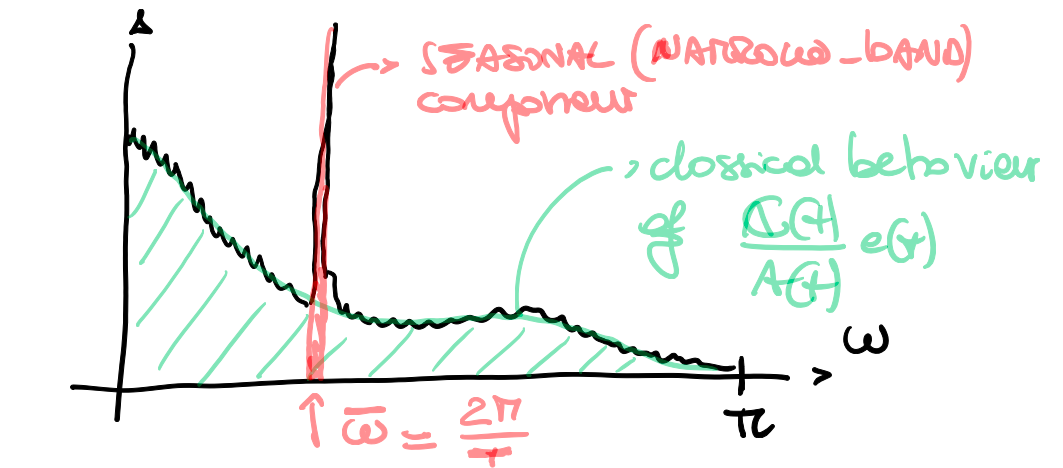
\includegraphics[width=.7\linewidth]{seasonal_fft}
\end{figure}
\item s(t) is \textbf{not a trend} $\to$  the process (raw data) y(t) can have \textbf{both} a trend and a seasonal behaviour. \textbf{FIRST} remove the trend \textbf{THEN} the seasonal behaviour.
\item If we don't remove a seasonal behaviour we end up with an ARMA model having a pair of complex conjugate poles at:
$$ e^{\pm j\Omega} , \Omega =\frac{2\pi}{T}$$  
\end{itemize}
\end{description}
\par\noindent\rule{\textwidth}{0.4pt}
The seasonal component of raw data can be estimated :
$$ t=1,2,3...N \text{  ,  } M\cdot T \leq N$$
\[
\boxed{\frac{1}{M}\sum\limits_{h=0}^{M-1}y(t+hT) \text{  , t=1,2,3...N}}
\]
\begin{figure}[H]
 \centering
  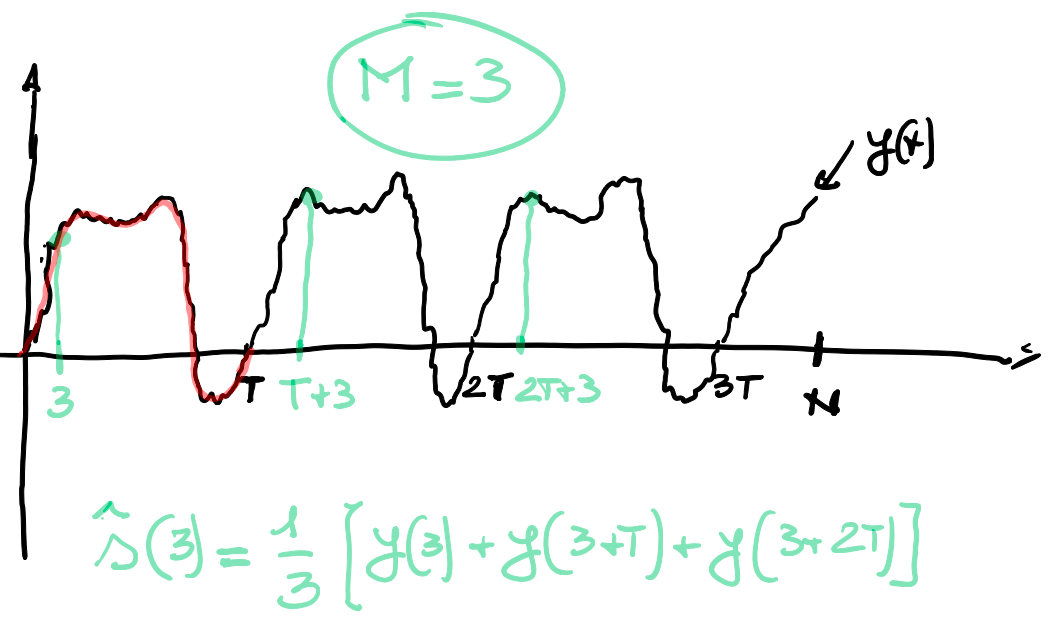
\includegraphics[width=.6\linewidth]{seasonal_est}
\end{figure}
\begin{figure}[H]
 \centering
  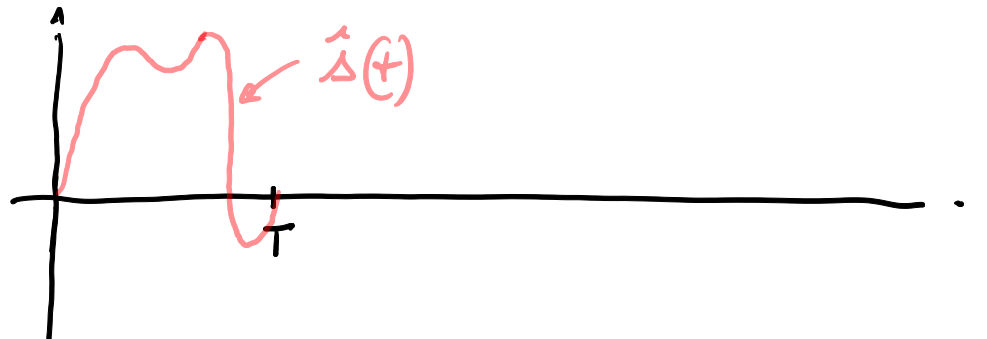
\includegraphics[width=.7\linewidth]{seasonal_est2}
\end{figure}
Once $\hat{s}$ is computed we can remove it from y(t).\\
After modelling $\tilde{y}(t)$ with an ARMA model the prediction will be:
\[
\boxed{\hat{y}(t+1|t) = \hat{\tilde{y}}(t+1|t) + \hat{s}(|t+1|_T)}
\]

\subsection{02-20-2013}
\textbf{Q:Give the definition of spectral density of a stochastic process y(t) and list its properties}
\vspace{2mm}\\
The spectral density describes the distribution of power into frequency components composing that signal.According to Fourier analysis any physical signal can be decomposed into a number of discrete frequencies, or a spectrum of frequencies over a continuous range. The statistical average of a certain signal or sort of signal (including noise) as analyzed in terms of its frequency content, is called its spectrum.
The \textbf{power density / spectral density / spectrum } of a \textbf{SSP} y(t) :
$$\Gamma_y(w) = \sum\limits_{\tau = -\infty}^{\infty} \gamma_y(\tau)e^{-jw\tau}$$
where $\Gamma_y(w)$ is the \textbf{Discrete Fourier Transform}.\\
Properties :
\begin{enumerate}
\item $\Gamma_y(w)$ is a \textbf{real} function of a \textbf{real} variable w which means that $Im\{\Gamma_y(w)\}=0$
\item $\Gamma_y(w)$ is a \textbf{positive} function which means that $\Gamma_y(w) \geq 0 , \forall w \in \Re$
\item $\Gamma_y(w)$ is an \textbf{even} function which means that $\Gamma_y(w) =\Gamma_y(-w)$
\item $\Gamma_y(w)$ is a \textbf{periodic} function of period $2\pi$ which means that $\Gamma_y(w) = \Gamma_y(w+k-2\pi)$.
\end{enumerate}
\vspace{8mm}
\textbf{Q:Prove (the complete proof is required) that if }$S \in M(\theta)$, \textbf{a P.E.M.  method can guarantee that the estimated model is the true model asymptotically.}\vspace{2mm}\\
Lets assume that the \textbf{real system S} that has generated the dataset is within the model class : $ \text{\textbf{S}} \in m(\theta) \to a\theta ^0$  exists so that $ m(\theta^0) = \text{\textbf{S}}$.
$$ \text{Is } \theta^0 = \bar{\theta} \text{?}$$
In other words , is the P.E.M performance index able to select the \textbf{true} parameter $\theta^0$?
\begin{description}
\item[Proof]\hfill\\
Consider the prediction error $\epsilon(t,\theta) = y(t) - \hat{y}(t|t-1,\theta)$.
Add on both sides $ -\hat{y}(t|t-1,\theta^0)$:
$$ \epsilon(t,\theta) -\hat{y}(t|t-1,\theta^0) = y(t) - \hat{y}(t|t-1,\theta) -\hat{y}(t|t-1,\theta^0)$$
Where $y(t)-\hat{y}(t|t-1,\theta^0)$ is the \textbf{white noise} e(t) of the true system \textbf{S}.
$$ \epsilon(t,\theta)=e(t)-(\hat{y}(t|t-1,\theta^0)-\hat{y}(t|t-1,\theta))$$
Square and apply expected value:
$$ E[\epsilon(t,\theta)^2]=E[e(t)^2]+E[(\hat{y}(t|t-1,\theta^0)-\hat{y}(t|t-1,\theta))^2]+2E[e(t)(\hat{y}(t|t-1,\theta^0)-\hat{y}(t|t-1,\theta))]$$
The last term is =0 because e(t) cannot be correlated with $\hat{y}(t|t-1,\theta)$ or $\hat{y}(t|t-1,\theta^0)$. Remembering that $E[\epsilon(t,\theta)^2]= \bar{J}(\theta)$ and $E[e(t)^2]=var[e(t)] = \lambda^2$ :
$$ \bar{J}(\theta) = \lambda^2 + E[(\hat{y}(t|t-1,\theta^0)-\hat{y}(t|t-1,\theta))^2]$$
\[  E[(\hat{y}(t|t-1,\theta^0)-\hat{y}(t|t-1,\theta))^2]=
  \begin{cases}
    \geq 0       & \quad \text{if } \theta \neq \theta^0\\
   	 0  			 & \quad \text{if } \theta = \theta^0
  \end{cases}
\]
So $\bar{J}(\theta) \geq \lambda^2 = \bar{J}(\theta^0)$ which means that $\theta^0$ is the global minimum of $\bar{J}(\theta) $ $$ \bar{\theta} = \theta^0$$ The P.E.M provides the \textbf{true model} if \textbf{S} $\in m(\theta)$ 
\end{description}
\end{document}
